\section*{Цель работы}
Исследовать характеристики фоторезистора при внутреннем фотоэффекте; найти ширину запрещенной зоны полупроводника.

\section*{Приборы и принадлежности}
Модульный учебный комплекс МУК-ОК, в состав которого входят стенд с объектами исследования С3-ОК01, амперметр-вольтметр АВ-1, источник питания ИПС1, соединительные проводники.

\section*{Исследуемые закономерности}
\textit{Принцип действия фоторезистора} (фотосопротивления) основан на изменении фотопроводимости полупроводника под действием света (явление внутреннего фотоэффекта). В основе внутреннего фотоэффекта лежит переход электронов из связанных состояний в свободные при поглощении квантов светового излучения. В результате этого в полупроводниках образуются электронно-дырочные пары: освобожденный от валентной связи электрон, способный перемещаться по кристаллу, и дырка.

Удельная фотопроводимость полупроводника определяется как разность между удельной проводимостью при освещении и в темноте:
$$ \Delta\sigma_\text{ф} = \sigma_\text{осв} - \sigma_\text{т} = e (\mu_n \Delta n + \mu_p \Delta p) $$
где $e$ — заряд электрона; $\mu_n$ и $\mu_p$ — подвижности электронов и дырок; $\Delta n$ и $\Delta p$ — концентрации избыточных электронов и дырок.

В данной лабораторной работе исследуются следующие основные характеристики фоторезистора:

\begin{enumerate}
    \item \textit{Вольт-амперной характеристикой} называется зависимость фототока $I_\text{ф}$, протекающего через фоторезистор, от приложенного напряжения $U$ при постоянном световом потоке $\Phi$:
          $$ I_\text{ф} = f(U)|_{\Phi=\text{const}, \lambda=\text{const}} $$
          Амперметр в схеме установки регистрирует полный ток $I$, включающий в себя темновой ток $I_\text{т}$ и фототок $I_\text{ф}$:
          $$ I = I_\text{т} + I_\text{ф} $$

    \item \textit{Световой характеристикой} называется зависимость фототока $I_\text{ф}$ от падающего светового потока $\Phi$ при постоянном значении приложенного напряжения $U$.
          $$ I_\text{ф} = f(\Phi)|_{U=\text{const}} $$
          Характерный вид кривой приведен на \cref{fig:light_char}.

    \item \textit{Спектральной характеристикой} называется зависимость фототока $I_\text{ф}$ от длины волны $\lambda$ при постоянном световом потоке.
          Характерный вид кривой приведен на \cref{fig:spectral_char}.
\end{enumerate}

Определив по спектральной характеристике край собственного поглощения (красную границу фотоэффекта) $\lambda_\text{кр}$, можно оценить ширину запрещенной зоны полупроводника $\Delta\varepsilon$:
$$ \Delta\varepsilon = \frac{hc}{\lambda_\text{кр}} $$

\begin{figure}[H]
    \centering
    \begin{minipage}{0.48\linewidth}
        \centering
        \def\thefigure{7.7}
        \protect\phantomsection
        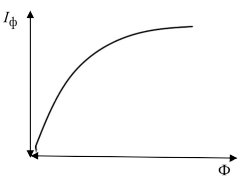
\includegraphics[width=0.9\linewidth]{figs/7-7.png}
        \caption{Световая характеристика фоторезистора}
        \label{fig:light_char}
    \end{minipage}\hfill
    \begin{minipage}{0.48\linewidth}
        \centering
        \def\thefigure{7.8}
        \protect\phantomsection
        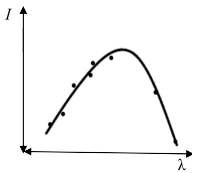
\includegraphics[width=0.9\linewidth]{figs/7-8.png}
        \caption{Спектральная характеристика фоторезистора}
        \label{fig:spectral_char}
    \end{minipage}
\end{figure}

\newpage
\centeredsection{\MakeUppercase{Указания по проведению эксперимента}}

\begin{figure}[H]
    \centering
    \begin{minipage}{0.48\linewidth}
        \centering
        \def\thefigure{7.5}
        \protect\phantomsection
        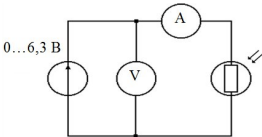
\includegraphics[width=0.9\linewidth]{figs/7-5.png}
        \caption{Электрическая схема экспериментальной установки}
        \label{fig:circuit}
    \end{minipage}\hfill
    \begin{minipage}{0.48\linewidth}
        \centering
        \def\thefigure{7.6}
        \protect\phantomsection
        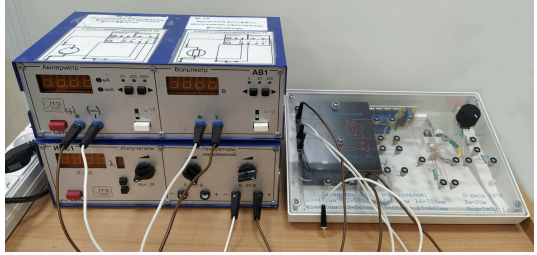
\includegraphics[width=0.9\linewidth]{figs/7-6.png}
        \caption{Модульный учебный комплекс МУК-ОК}
        \label{fig:setup}
    \end{minipage}
\end{figure}

\begin{enumerate}
    \item \textbf{Собрать электрическую схему} с помощью коммутации проводников (см. \cref{fig:circuit}).

    \item \textbf{Включить приборы.} На блоке управления ИПС1 регулятором интенсивности излучения установить значение $J/J_0$ в диапазоне $1.0...1.2$; выбрать режим измерения вольтметра ($6.3$ В) и амперметра ($200$ мкА).

    \item \textbf{Снять темновую характеристику} фоторезистора $I_\text{т} = f(U)_{\Phi=\text{const}}$ при $\Phi = J/J_0 = 0.1$ с шагом изменения напряжения $\Delta U = 0.5$ В. Значения занести в \cref{tab:protocol_V-A}.

    \item \textbf{Снять семейство вольт-амперных характеристик} (зависимость фототока $I_\text{ф} = I - I_\text{т}$ от напряжения $U$) для трех значений длины волны $\lambda$ при фиксированном значении $\Phi = J/J_0$ с шагом изменения напряжения $\Delta U = 0.5$ В. Значения $\lambda_1, \lambda_2, \lambda_3$ и $\Phi$ задаются преподавателем. Результаты измерений занести в \cref{tab:protocol_V-A}. Рассчитать для каждого значения напряжения $U$ истинное значение фототока.

    \item \textbf{Снять семейство световых характеристик} (зависимость фототока от светового потока $\Phi = J/J_0$). Измерения выполнить при фиксированном напряжении $U$ для двух длин волн с шагом по $J/J_0 = 0.1$. Фиксированные значения $U, \lambda_1$ и $\lambda_2$ задаются преподавателем. Результаты измерений занести в \cref{tab:protocol_light}.

    \item \textbf{Снять спектральную характеристику} фотоэлемента, используя все 8 длин волн. Измерения выполнять при фиксированных значениях напряжения $U$ и светового потока $\Phi = J/J_0$, задаваемых преподавателем. Результаты измерений занести в \cref{tab:protocol_spectral}.
\end{enumerate}

\newpage
\thispagestyle{empty}
\centeredsection{ПРОТОКОЛ НАБЛЮДЕНИЙ}

\begin{table}[H]
    \centering
    \caption{Вольт-амперные характеристики фоторезистора ($I_\text{ф} = f(U)_{\Phi=\text{const}, \lambda=\text{const}}$), $J/J_0 = \rule{1.5cm}{0.4pt}$}
    \label{tab:protocol_V-A}
    \begin{tabularx}{\linewidth}{|c|c|*{12}{C|}}
        \hline

        \multicolumn{2}{|c|}{\multirow{2}{*}{Параметр}}  & \multicolumn{12}{c|}{Напряжение $U$, В}                                                         \\
        \cline{3-14}
        \multicolumn{2}{|c|}{}                           & 0.5                                     & 1 & 1.5 & 2 & 2.5 & 3 & 3.5 & 4 & 4.5 & 5 & 5.5 & 6   \\

        \hline \hline

        \multicolumn{2}{|c|}{$I_\text{т}$}               &                                         &   &     &   &     &   &     &   &     &   &     &     \\

        \hline \hline

        \multirow{2}{*}{$\lambda_1 = \rule{1cm}{0.4pt}$} & $I$                                     &   &     &   &     &   &     &   &     &   &     &   & \\
        \cline{2-14}
                                                         & $I_\text{ф}$                            &   &     &   &     &   &     &   &     &   &     &   & \\


        \hline \hline

        \multirow{2}{*}{$\lambda_2 = \rule{1cm}{0.4pt}$} & $I$                                     &   &     &   &     &   &     &   &     &   &     &   & \\
        \cline{2-14}
                                                         & $I_\text{ф}$                            &   &     &   &     &   &     &   &     &   &     &   & \\

        \hline \hline

        \multirow{2}{*}{$\lambda_3 = \rule{1cm}{0.4pt}$} & $I$                                     &   &     &   &     &   &     &   &     &   &     &   & \\
        \cline{2-14}
                                                         & $I_\text{ф}$                            &   &     &   &     &   &     &   &     &   &     &   & \\

        \hline
    \end{tabularx}
\end{table}

\begin{table}[H]
    \centering
    \caption{Световые характеристики фоторезистора ($I_\text{ф} = f(\Phi)_{U=\text{const}}$), $U = \rule{1.5cm}{0.4pt}$ В, $I_\text{т} = \rule{1.5cm}{0.4pt}$ мкА}
    \label{tab:protocol_light}
    \begin{tabularx}{\linewidth}{|c|l|*{13}{C|}}
        \hline
        \multicolumn{2}{|c|}{\multirow{2}{*}{Параметр}}  & \multicolumn{13}{c|}{Относительный световой поток $J/J_0$}                                                                           \\
        \cline{3-15}
        \multicolumn{2}{|c|}{}                           & 0                                                          & 0.1 & 0.2 & 0.3 & 0.4 & 0.5 & 0.6 & 0.7 & 0.8 & 0.9 & 1.0 & 1.1 & 1.2   \\
        \hline \hline
        \multirow{2}{*}{$\lambda_1 = \rule{1cm}{0.4pt}$} & $I$                                                        &     &     &     &     &     &     &     &     &     &     &     &     & \\
        \cline{2-15}
                                                         & $I_\text{ф}$                                               &     &     &     &     &     &     &     &     &     &     &     &     & \\
        \hline \hline
        \multirow{2}{*}{$\lambda_2 = \rule{1cm}{0.4pt}$} & $I$                                                        &     &     &     &     &     &     &     &     &     &     &     &     & \\
        \cline{2-15}
                                                         & $I_\text{ф}$                                               &     &     &     &     &     &     &     &     &     &     &     &     & \\
        \hline
    \end{tabularx}
\end{table}

\begin{table}[H]
    \centering
    \caption{Спектральная характеристика фоторезистора ($I_\text{ф} = f(\lambda)_{\Phi=\text{const}}$), $J/J_0 = \rule{1.5cm}{0.4pt}$, $U = \rule{1.5cm}{0.4pt}$ В, $I_\text{т} = \rule{1.5cm}{0.4pt}$ мкА}
    \label{tab:protocol_spectral}
    \begin{tabularx}{\linewidth}{|c|*{8}{C|}}
        \hline
        $\lambda$ & 430 & 470 & 520 & 565 & 590 & 660 & 700 & 860 \\
        \hline \hline
        $I$                   &     &     &     &     &     &     &     &     \\
        \hline
        $I_\text{ф}$          &     &     &     &     &     &     &     &     \\
        \hline
    \end{tabularx}
\end{table}

\textit{Примечание: } $[\lambda_\forall] = [\text{нм}]$; \hfill $[I_\forall] = [\text{мкА}]$; \hfill $I_\text{ф} = I - I_\text{т}$

\vfill
\noindent
Рахметов А. Р., гр. 4494 ~~\hrulefill~~ «\rule{1cm}{0.4pt}» \rule{3cm}{0.4pt} 20\rule{0.75cm}{0.4pt} г.